\chapter{The SVD, PCA, and Low-Rank Approximation}
\label{ch:svd-pca-low-rank}

\section{What Replaces Diagonalization?}

Eigenvalue decomposition is built for square matrices, and the best version of
it belongs to symmetric matrices:
\[
  A=Q\Lambda Q^T.
\]
Most data matrices are not square or symmetric. A data matrix might have rows
as samples and columns as features. An image might be a rectangular matrix of
pixel intensities. A linear map may go from $\R^n$ to $\R^m$ with $m\neq n$.

The singular value decomposition is the replacement:
\[
  A=U\Sigma V^T.
\]
It works for every real matrix.

\section{\texorpdfstring{From $A^TA$ To Singular Values}{From A Transpose A To Singular Values}}

Let $A\in\R^{m\times n}$. The matrix $A^TA$ is symmetric PSD, so the spectral
theorem gives an orthonormal eigenbasis
\[
  v_1,\ldots,v_n
\]
with eigenvalues
\[
  \lambda_1\geq\lambda_2\geq\cdots\geq\lambda_n\geq 0.
\]

\begin{definition}[Singular values and right singular vectors]
The \emph{singular values} of $A$ are
\[
  \sigma_i=\sqrt{\lambda_i}.
\]
The eigenvectors $v_i$ of $A^TA$ are the \emph{right singular vectors}.
\end{definition}

For any right singular vector,
\[
  \norm{Av_i}^2
  =
  v_i^TA^TAv_i
  =
  \lambda_i
  =
  \sigma_i^2.
\]
Thus $\sigma_i$ measures how much $A$ stretches the input direction $v_i$.

\section{Left Singular Vectors}

If $\sigma_i>0$, define
\[
  u_i=\frac{Av_i}{\sigma_i}.
\]
Then
\[
  Av_i=\sigma_i u_i.
\]

\begin{proposition}
For the positive singular values, the vectors $u_i$ are orthonormal.
\end{proposition}

\begin{proof}
For $i=j$,
\[
  \norm{u_i}^2
  =
  \frac{\norm{Av_i}^2}{\sigma_i^2}
  =
  1.
\]
For $i\neq j$,
\[
  \inner{u_i}{u_j}
  =
  \frac{(Av_i)^T(Av_j)}{\sigma_i\sigma_j}
  =
  \frac{v_i^TA^TAv_j}{\sigma_i\sigma_j}
  =
  \frac{\sigma_j^2 v_i^Tv_j}{\sigma_i\sigma_j}
  =
  0.
\]
\end{proof}

The remaining $u_i$ can be chosen to complete an orthonormal basis of
$\R^m$.

\section{The SVD Theorem}

\begin{theorem}[Singular value decomposition]
For every matrix $A\in\R^{m\times n}$, there are orthogonal matrices
$U\in\R^{m\times m}$ and $V\in\R^{n\times n}$ and a rectangular diagonal
matrix $\Sigma\in\R^{m\times n}$ such that
\[
  A=U\Sigma V^T.
\]
The diagonal entries of $\Sigma$ are the singular values
\[
  \sigma_1\geq\sigma_2\geq\cdots\geq 0.
\]
\end{theorem}

The meaning is geometric:
\[
  \text{rotate/reflect by }V^T,
  \qquad
  \text{stretch by }\Sigma,
  \qquad
  \text{rotate/reflect by }U.
\]

\begin{figure}[htbp]
  \centering
  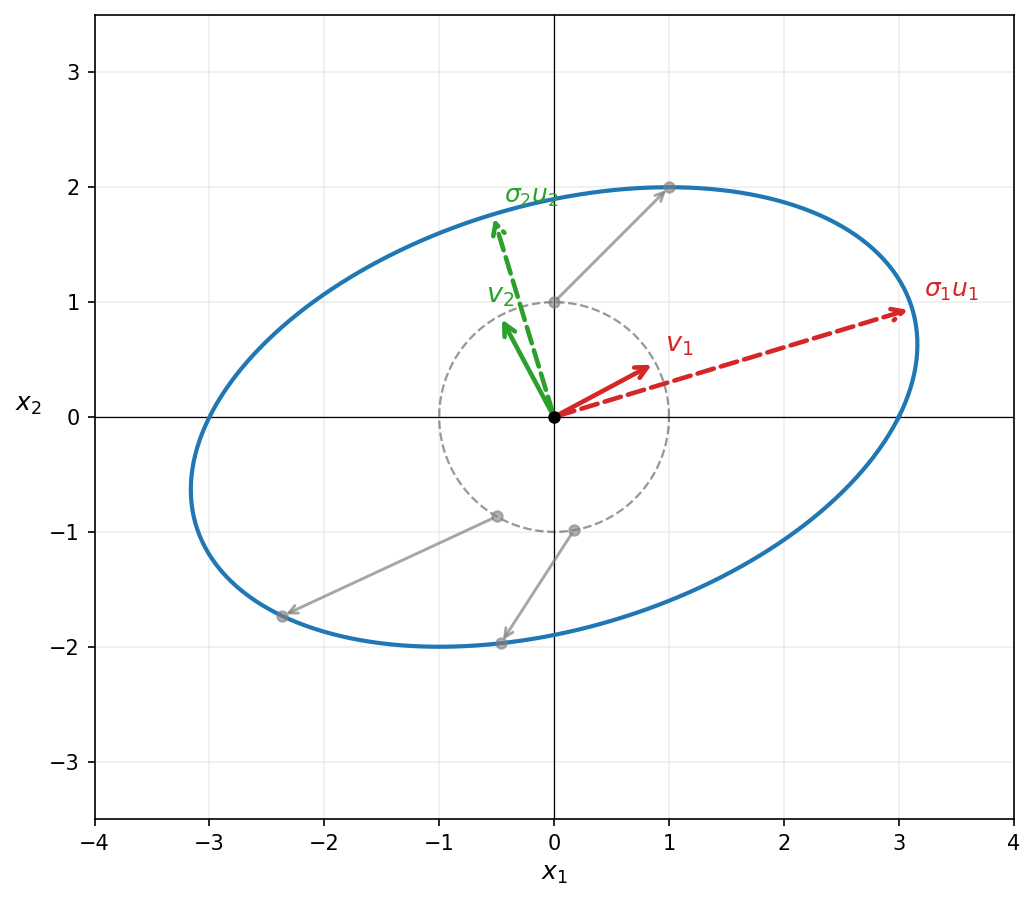
\includegraphics[width=0.70\textwidth]{book/assets/figures/core/fig09_svd_geometry.png}
  \caption{The SVD separates input directions $v_i$, output directions $u_i$,
  and stretch factors $\sigma_i$. A circle maps to an ellipse.}
\end{figure}

\section{Four Subspaces Through The SVD}

Let $r=\Rank(A)$. Then exactly $r$ singular values are positive. The SVD
organizes the four fundamental subspaces:
\[
  \row(A)=\Span(v_1,\ldots,v_r),
  \qquad
  \Ker(A)=\Span(v_{r+1},\ldots,v_n),
\]
\[
  \col(A)=\Span(u_1,\ldots,u_r),
  \qquad
  \Ker(A^T)=\Span(u_{r+1},\ldots,u_m).
\]
This is the geometric picture from Chapter~\ref{ch:projection-least-squares}
with orthonormal bases built in.

\section{Outer Products And Low Rank}

The SVD can be written as a sum of rank-one matrices:
\[
  A=\sigma_1u_1v_1^T+\sigma_2u_2v_2^T+\cdots+\sigma_ru_rv_r^T.
\]
The rank-$k$ truncation keeps only the first $k$ terms:
\[
  A_k=\sum_{i=1}^k \sigma_i u_i v_i^T.
\]

\begin{theorem}[Eckart--Young, statement]
Among all matrices of rank at most $k$, the truncated SVD $A_k$ is closest to
$A$ in Frobenius norm:
\[
  A_k=\operatorname*{argmin}_{\Rank(B)\leq k}\norm{A-B}_F.
\]
Moreover,
\[
  \norm{A-A_k}_F^2=\sigma_{k+1}^2+\cdots+\sigma_r^2.
\]
\end{theorem}

The error formula is easy to remember: the squared Frobenius error is the sum
of the squared singular values you throw away.

\begin{figure}[htbp]
  \centering
  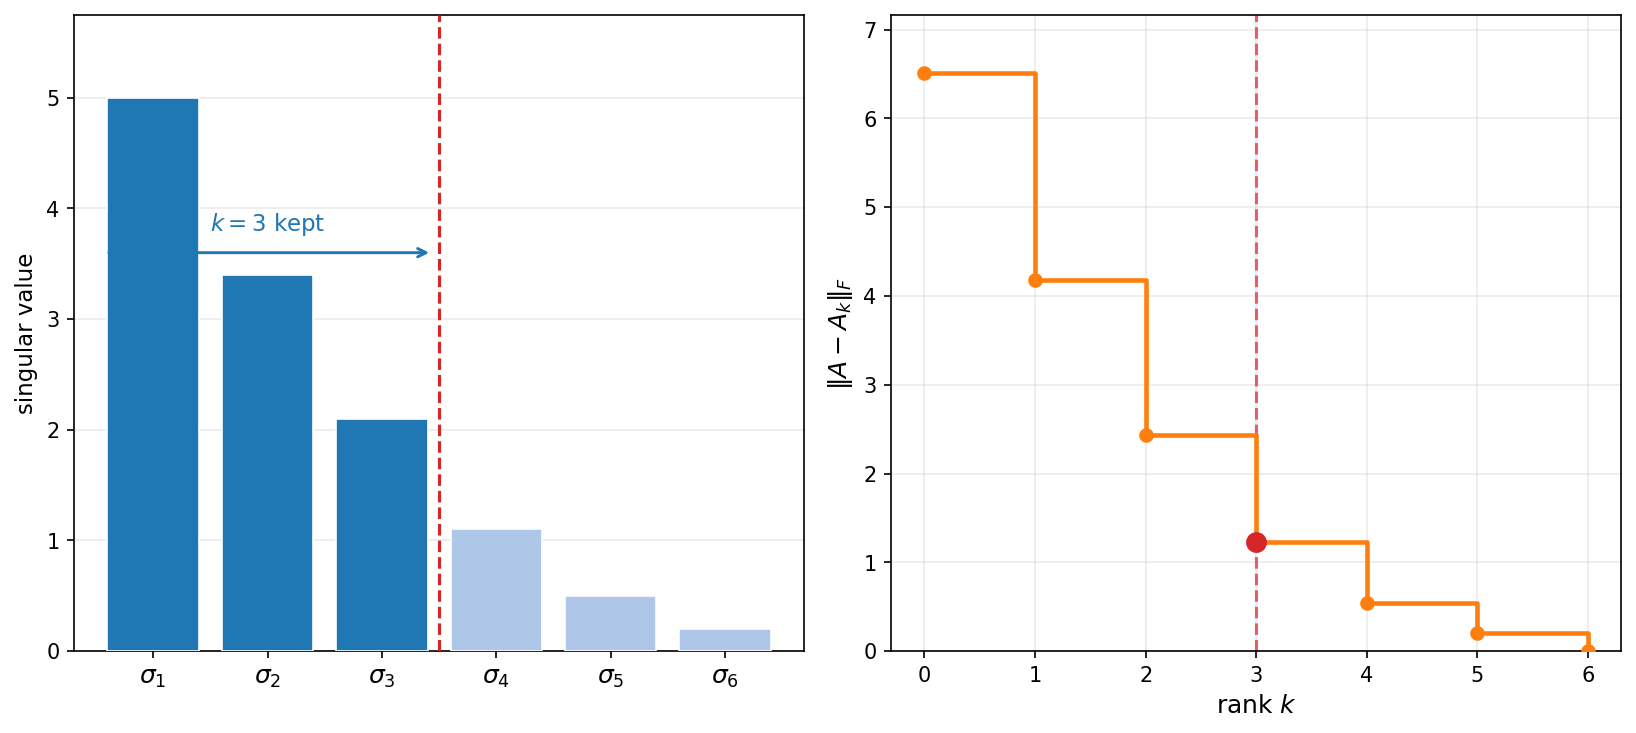
\includegraphics[width=0.92\textwidth]{book/assets/figures/core/fig10_eckart_young.png}
  \caption{Low-rank approximation keeps the largest singular values and
  discards the tail. The discarded tail determines the Frobenius error.}
\end{figure}

\begin{aimlbox}
Low-rank approximation is not an ``AI trick.'' It is a geometric theorem about
matrices. It becomes useful in data work because many datasets have dominant
directions or repeated structure, so a small number of singular directions
captures much of the matrix.
\end{aimlbox}

\section{PCA As SVD Of Centered Data}

Let $X\in\R^{N\times d}$ be a centered data matrix: rows are samples, columns
are features. The covariance matrix is
\[
  C=\frac{1}{N-1}X^TX.
\]
The right singular vectors of $X$ are the eigenvectors of $X^TX$, hence also
of $C$. These are the principal component directions.

If
\[
  X=U\Sigma V^T,
\]
then the columns of $V$ are principal directions, and the variance explained
by direction $v_i$ is proportional to $\sigma_i^2$.

\[
  \text{fraction explained by first }k
  =
  \frac{\sigma_1^2+\cdots+\sigma_k^2}
       {\sigma_1^2+\cdots+\sigma_r^2}.
\]

\begin{figure}[htbp]
  \centering
  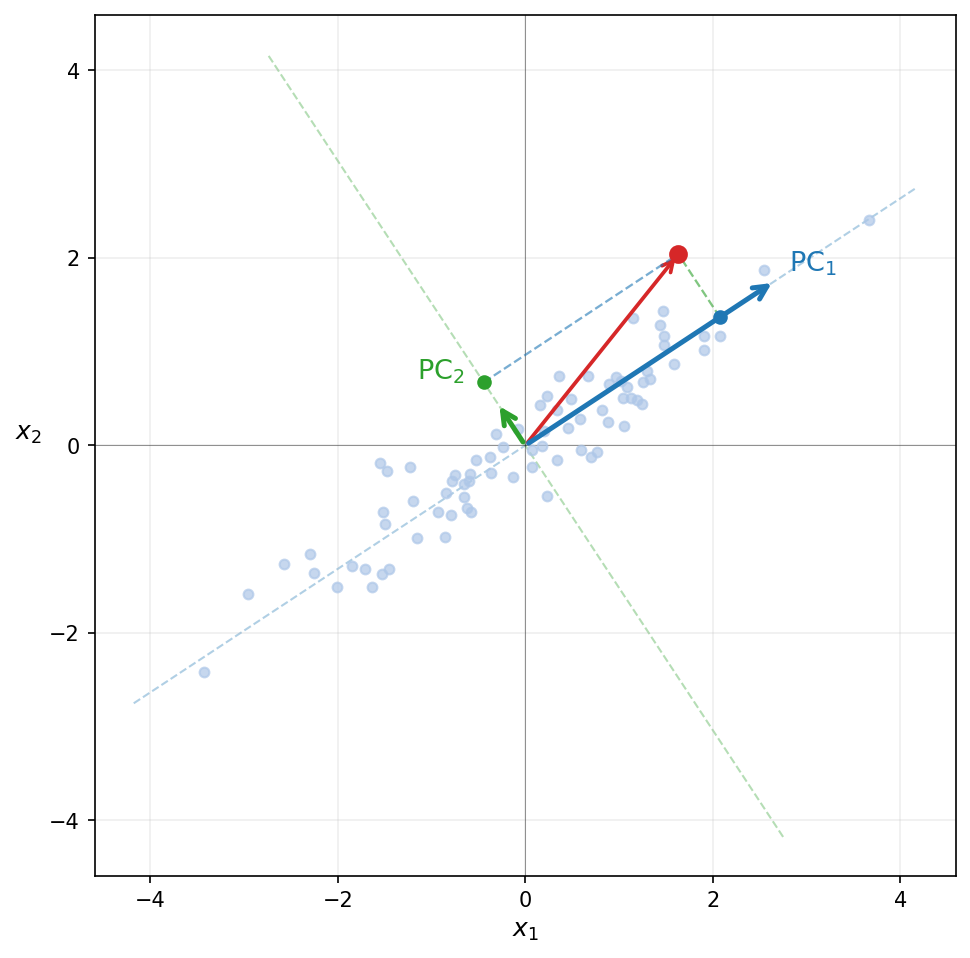
\includegraphics[width=0.72\textwidth]{book/assets/figures/core/fig11_pca.png}
  \caption{PCA finds orthogonal directions of decreasing variance. Projecting
  onto the first component gives the best one-dimensional linear summary.}
\end{figure}

\section{Python Thread}

\begin{lstlisting}
import numpy as np

rng = np.random.default_rng(0)
A = rng.standard_normal((4, 3))

U, s, Vt = np.linalg.svd(A, full_matrices=False)
A_reconstructed = U @ np.diag(s) @ Vt

print("reconstruction:", np.allclose(A, A_reconstructed))
print("singular values:", s)

# Rank-k approximation
k = 2
A_k = U[:, :k] @ np.diag(s[:k]) @ Vt[:k, :]
err = np.linalg.norm(A - A_k, "fro")
err_formula = np.sqrt(np.sum(s[k:]**2))
print("rank-k error:", err)
print("error formula:", err_formula)

# PCA on centered data
X = rng.standard_normal((100, 5))
X = X - X.mean(axis=0)
Ux, sx, Vtx = np.linalg.svd(X, full_matrices=False)
variance_fraction = sx**2 / np.sum(sx**2)
print("variance fractions:", variance_fraction)
print("first two total:", np.sum(variance_fraction[:2]))
\end{lstlisting}

\begin{labbox}
Lab 10 visualizes the SVD geometry and low-rank approximation. Lab 12 uses
truncated SVD for denoising. The book chapter keeps the core theorem visible;
the labs show what the singular values look like in computation.
\end{labbox}

\section*{Chapter Summary}
\addcontentsline{toc}{section}{Chapter Summary}

\begin{itemize}
  \item $A^TA$ is symmetric PSD, so its eigenvectors define right singular
        directions.
  \item Singular values measure stretch factors.
  \item The SVD writes every real matrix as $A=U\Sigma V^T$.
  \item The SVD gives orthonormal bases for the four fundamental subspaces.
  \item Truncated SVD gives the best low-rank approximation in Frobenius norm.
  \item PCA is SVD applied to centered data.
\end{itemize}

\section*{Exercises}
\addcontentsline{toc}{section}{Exercises}

\subsection*{A. Theory}

\begin{exercise}
\exerciseid{14.A1}
Explain why $A^TA$ is symmetric and PSD for any real matrix $A$.
\end{exercise}

\begin{exercise}
\exerciseid{14.A2}
Explain, without proving the full Eckart--Young theorem, why a low-rank
approximation should keep the largest singular values first.
\end{exercise}

\subsection*{B. By Hand}

\begin{exercise}
\exerciseid{14.B1}
Find an SVD of the diagonal matrix
\[
  \begin{bmatrix}3&0\\0&1\end{bmatrix}.
\]
\end{exercise}

\begin{exercise}
\exerciseid{14.B2}
For singular values $8,3,1$, compute the squared Frobenius-norm error of the
best rank-$1$ approximation and of the best rank-$2$ approximation.
\end{exercise}

\subsection*{C. Python / NumPy}

\begin{exercise}
\exerciseid{14.C1}
Use \texttt{np.linalg.svd} to reconstruct a random $4\times 3$ matrix.
\end{exercise}

\begin{exercise}
\exerciseid{14.C2}
Center a small data matrix by subtracting column means, compute its SVD, and
report how much variance is captured by the first singular direction.
\end{exercise}

\begin{exercise}
\exerciseid{14.C3}
For a random $6\times 4$ matrix, compute rank-$k$ approximations for
$k=1,2,3$. Compare the measured Frobenius error with the formula using
discarded singular values.
\end{exercise}

\subsection*{D. Challenge}

\begin{exercise}
\exerciseid{14.D1}
Explain what singular values measure geometrically for a $2\times 2$ matrix.
\end{exercise}

